\chapter{Experiment}
\label{chap:experiment}

We have incorporated our algorithm to the software model checker for
higher-order programs \textsc{MoCHi} \cite{conf/pldi/KobayashiSU11}.  It is
specifically designed to verify the correctness of higher-order
programs written in a small subset of ML.  This verification tool
abstracts a given input program by inferring dependent types for
higher-order programs \cite{conf/ppdp/UnnoK09}.

We implemented our proposed algorithm into \textsc{MoCHi} by two steps.  First,
we replace an existing theorem prover with our interpolating theorem
prover as a sub-routine for solving Horn clauses in dependent typing.
We used a method to obtain a common small interpolant across different
interpolating problems, while reducing a Horn clause problem into
interpolation \cite{conf/ppdp/UnnoK09}.  Second, we completely
replaced \textsc{MoCHi}'s Horn solving algorithm with our algorithm.

For simplicity of the implementation, we assume that the linear
inequalities in the integer space.  Because of this, our algorithm
lost the completeness.  By using Motzkin's transpose theorem
\cite{journals/networks/Rajan90}, it is possible to handle linear
inequalities in both $\mathbf{ax} + b \leq 0$ and $\mathbf{ax} + b <
0$.

While solving interpolating problems, our algorithm treated linear
equalities in the form $\mathbf{ax} + b = 0$ specially without
normalizing into a conjunction of linear equalities so that the
algorithm obtain a linear equality in a set of interpolants.  It is
because we observed some cases that require an equality relation
between two variables but not an inequality as an program invariant.

Note that, however, in Horn clauses solving problems, when a predicate
variable $P$ needs to take an equality $=$ or negation $\neq$, the
predicate template grows during the solving process as
$\mathbf{ax}-b \leq 0 \wedge -\mathbf{ax}+b \leq 0$ in the former
case, and $\mathbf{ax}-b+1 \leq 0 \vee -\mathbf{ax}+b+1 \leq 0$ in the
latter case.  We also thought it possible to obtain predicates that
are similar to program invariants by considering multiple paths.

For linear constraint satisfaction, we used GNU Linear Programming Kit
(GLPK) first for its light computation load.  For Horn clause solving
however, our implementation make use of Z3 \cite{conf/tacas/MouraB08}
as an SMT solver to obtain unsatisfiable core of the constraints.

\section{Interpolating theorem prover}

As an experiment of our interpolating algorithm, we compared the
quality of resulting interpolants with
ones that \textsc{CSIsat} \cite{conf/cav/BeyerZM08} generates.
It combines linear arithmetic reasoning and SAT-based logical reasoning.
\textsc{CSIsat} is mainly used as a sub procedure of current \textsc{MoCHi}.  Note that
it may return different interpolants for an interpolating problem
because of the randomized algorithm.  Results shown below
are ones that are randomly chosen.
\textsc{Yint} represents our interpolating algorithm.

\begin{itemize}
\item Disjunctive interpolation in $A$.
\[\begin{array}{r c}
\varphi_A : & (x-1 \geq 0) \vee (x+1 \leq 0) \\
\hline
\varphi_B : & x=0
\end{array}\]
The result for this:
\[\begin{array}{l c}
\text{\textsc{Yint}} & (x+1 \leq 0) \vee (-x+1 \leq 0) \\
\text{\textsc{CSIsat}} & (-x \leq -1 \vee x \leq -1)
\end{array}\]
\item Disjunctive interpolation in $B$.
\[\begin{array}{r c}
\varphi_A : & x=0 \\
\hline
\varphi_B : & (x-1 \geq 0) \vee (x+1 \leq 0)
\end{array}\]
\[\begin{array}{l c}
\text{\textsc{Yint}} & -x=0 \\
\text{\textsc{CSIsat}} & (-x \leq 0 \wedge x \leq 0)
\end{array}\]
\item Complex formula in $A$.
% complicated disj
\[\begin{array}{r c}
\varphi_A : & ((x-5<0) \wedge (-x<0)) \vee ((x<0) \wedge (-x-5<0)) \\
\hline
\varphi_B : & x=0
\end{array}\]
\[\begin{array}{l c}
\text{\textsc{Yint}} & (x+1 \leq 0) \vee (-x+1 \leq 0) \\
\text{\textsc{CSIsat}} & (x < 0 \vee -x < 0)
\end{array}\]
\end{itemize}
For those problems that are simple enough, \textsc{Yint} and \textsc{CSIsat} returns the
same results.

Next we tried the problem that an equality interpolant exists.
% equality
\[\begin{array}{r c}
\varphi_A : & x=0 \\
\hline
\varphi_B : & x-1=0
\end{array}\]
\[\begin{array}{l c}
\text{\textsc{Yint}} & x=0 \\
\text{\textsc{CSIsat}} & x \leq 0
\end{array}\]

\bigskip\centerline{}

% quantifier
\[\begin{array}{r c}
\varphi_A : & (y-z=0) \wedge (x-z=0) \\
\hline
\varphi_B : & (-w+y+1 \leq 0) \wedge (-w+x \geq 0)
\end{array}\]
\[\begin{array}{l c}
\text{\textsc{Yint}} & x-y=0 \\
\text{\textsc{CSIsat}} & x-y \leq 0
\end{array}\]
Because our algorithm handles linear equalities special, our algorithm
makes an effort to return an interpolant of linear equality if one
exists.

Additionally, as the follwing results of \textsc{Yint} shows, if a
simple interpolant exists for a given problem, our algorithm tries
such result.
\[\begin{array}{r c}
\varphi_A : & ((-y+1 \leq 0) \wedge (-x \leq 0)) \vee ((-y \leq 0) \wedge (-x+1 \leq 0)) \\
\hline
\varphi_B : & ((y+1<0) \wedge (x<0)) \vee ((y<0) \wedge (x+1<0))
\end{array}\]
\[\begin{array}{l c}
\text{\textsc{Yint}} & -x \leq 0 \\
\text{\textsc{CSIsat}} & (((x < 0 \vee -x \leq 0) \wedge 0 \leq x) \vee ((y < 0 \vee -y \leq 0) \wedge 0 \leq y))
\end{array}\]

\bigskip\centerline{}

\[\begin{array}{r c}
\varphi_A : & (x-1=0) \vee (x+1=0) \\
\hline
\varphi_B : & (x-2=0) \vee (x=0) \vee (x+2=0)
\end{array}\]
\[\begin{array}{l c}
\text{\textsc{Yint}} & (-x-1=0) \vee (-x+1=0) \\
\text{\textsc{CSIsat}} & ((-x \leq -1 \vee x \leq -1) \wedge (-x \leq 1 \vee - x \leq - 1) \wedge (x \leq - 1 \vee x \leq 1))
\end{array}\]

\begin{figure}
\begin{center}
\includegraphics[scale=1.1]{figures/int1.eps}
\end{center}
\caption{Complex problem 1}
\label{fig:int1}
\end{figure}

Finally, we showed some test cases that may occur in practical interpolation.
\begin{itemize}
\item Problem in Figure~\ref{fig:int1}
\[\begin{array}{r c}
\multirow{2}{*}{$\varphi_A$}
& ((x-y-1 \leq 0) \wedge (-x+y-2 \leq 0) \wedge (x+y-1 \leq 0) \wedge (-x-y-2 \leq 0)) \vee \\
& ((x-y-2 \leq 0) \wedge (-x+y-1 \leq 0) \wedge (x+y-2 \leq 0) \wedge (-x-y-1 \leq 0)) \\
\hline
\varphi_B : & (x=0 \wedge y=2) \vee (x=0 \wedge y=-2)
\end{array}\]
\[\begin{array}{l c}
\text{\textsc{Yint}} & (-x+17y-33 \leq 0) \wedge (x-17y-33 \leq 0) \\
\text{\textsc{CSIsat}} & ((-1 \leq (x + y) \vee (x + -y) \leq 1) \wedge (-1 \leq (x + -y) \vee (x + y) \leq 1))
\end{array}\]

\item Problem in Figure~\ref{fig:int2}
\[\begin{array}{r c}
\multirow{2}{*}{$\varphi_A$}
& ((y+1=0) \wedge (x-1=0)) \vee ((y+1=0) \wedge (x+1=0)) \vee \\
& ((y-1=0) \wedge (x+1=0)) \vee ((y-1=0) \wedge (x-1=0)) \\
\hline
\multirow{2}{*}{$\varphi_B$}
& ((y+2 \leq 0) \wedge (x-2 \geq 0)) \vee ((y+2 \leq 0) \wedge (x+2 \leq 0)) \vee \\
& ((y-2 \geq 0) \wedge (x+2 \leq 0)) \vee ((y-2 \geq 0) \wedge (x-2 \geq 0))
\end{array}\]
\begin{tabular}{l c}
\textsc{Yint} & $(-2y-3 \leq 0) \wedge (2y-3 \leq 0)$
\end{tabular}

\textsc{CSIsat}
\begin{align*}
& ((-y \leq 1 \wedge y \leq -1) \vee (-y \leq -1 \wedge x \leq 1) \vee x \leq -1) \wedge \\
& \qquad (-x \leq 1 \vee -x \leq -1 \vee -y \leq -1) \wedge \\
& \qquad (-x \leq 1 \vee -x \leq -1 \vee y \leq -1) \wedge \\
& \qquad (-x \leq -1 \vee x \leq -1)
\end{align*}

\item Problem in Figure~\ref{fig:int3}
\[\begin{array}{r c}
\varphi_A & (x=1 \wedge y=1) \vee (x=0 \wedge y=0) \\
\hline
\varphi_B & (x=1 \wedge y \neq 1) \vee (x=0 \wedge y \neq 0)
\end{array}\]
\begin{tabular}{l c}
\textsc{Yint} & $x-y=0$
\end{tabular}

\textsc{CSIsat}
\begin{align*}
& ((((y \leq 0 \wedge -y \leq 0) \vee 1 = x) \wedge 1 \neq x) \vee ((1 \neq x \vee -y \leq -1) \wedge 1 = x) \vee 0 \neq x) \wedge \\
& \qquad (((0 \neq x \vee y \leq 1) \wedge (0 = x \vee y \leq 1)) \vee 1 \neq x) \wedge \\
& \qquad (((1 \neq x \vee -y \leq -1) \wedge 1 = x) \vee 0 = x) \wedge \\
& \qquad ((1 \neq x \wedge 1 = x) \vee (y \leq 0 \wedge -y \leq 0) \vee 0 \neq x) \wedge \\
& \qquad (1 = x \vee y \leq 0)
\end{align*}

\end{itemize}

\begin{figure}[htb]
  \begin{minipage}[t]{.47\textwidth}
  \centering
  \includegraphics[scale=1.1]{figures/int2.eps}
  \caption{Complex problem 2}
  \label{fig:int2}
  \end{minipage}
  \hfill
  \begin{minipage}[t]{.47\textwidth}
  \centering
  \includegraphics[scale=1.1]{figures/int3.eps}
  \caption{Complex problem 3}
  \label{fig:int3}
  \end{minipage}
\end{figure}


\section{Horn clause solving}

As an Horn clause solver we incorporated our Horn clause solver to
existing software model checker \textsc{MoCHi}.  It generates a Horn
clause solving problem while performing dependent type inference for
input program.

The previous \textsc{MoCHi} used Horn clause solving algorithm
proposed by Unno et al. \cite{conf/ppdp/UnnoK09}.  Its implementation
adopts \textsc{CSIsat} for solving interpolation problems that appear
as sub problems of Horn clause solving.

We configured \textsc{MoCHi} to use \textsc{TRecS} version 1.30 for
higher order model checking of abstract model of input programs.  The
experiments are performed for comparison between Unno's algorithm with
convex hull optimization in predicates (\texttt{-gchi} option) and our
algorithm (\texttt{-yhorn} option).  The test cases are available in
\textsc{MoCHi}'s development repository or online web interface.

For each test program, we compared the number of CEGAR cycles for
verification.  Additionally, for each Horn clause solving problem, we
inspected the quality of solutions.  The quality is evaluated by the
number of conjunctions and disjunctions in total.  Finally, we
compared the time consumed for solving each problem.


%\begin{figure}
%\begin{center}
%\includegraphics[scale=.8]{figures/time.eps}
%\end{center}
%\caption{Time consumption ration of Yhorn compared to \textsc{CSIsat}}
%\end{figure}

However we take a longer time for solving the same Horn clauses, which
means further optimization is required for our algorithm.
